\documentclass[11pt,a4paper]{article}
\title{APG4005F Assignment 2 Report}
\date{20 April 2015}
\author{Tim Marsh}

\usepackage{amsmath}
\usepackage{graphicx}
\usepackage{float}

\graphicspath{ {./} }
\begin{document}
	
	\pagenumbering{gobble}
	\maketitle
	\newpage
	\pagenumbering{arabic}
	\tableofcontents
	\listoffigures
	\newpage
	
	
	\section{Introduction}
	
	The primary objective for this assignment was to compare the difference between a Parametric and Free Network adjustment. the free network would be constrained using an S-Transform.
	
	An S-Transform makes it possible to transform the x-Vector and Q-Matrix of a free network adjustment into any minimum constrained datum and visa versa.
	
	In the case of this assignment i created 6 points (named A,B,C,D,P,Q) and fabricated angle observations between them. For the two methods to be worth comparing to each other the same points must be held fixed.
	
	I decided to hold points A and D fixed.

	\begin{figure}[H]
	\centering
	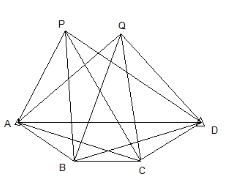
\includegraphics[width=0.5\linewidth]{./unnamed}
	\caption{Layout of Points}
	\label{fig:LayoutofPoints}
	\end{figure}

	
	\section{Background to the Problem}
	
	In a parametric adjustment of a survey network points must be held fixed so that the network can be adjusted to fit those points. If there are no points held fixed it will become impossible to solve the least squares adjustment because there will be a rank defect in the $A^TPA$ Matrix. This means that $A^TPA$ is singular and therefore not invertible.
	
	A free network does exactly that. Keeps no points fixed and winds up with a singular $A^TPA$ Matrix. it however solves this by introducing the $G$ Matrix.
	
	The $G$ matrix contains the eigenvectors of $A^TPA$ for all eigenvalues $\lambda = 0$.
	
	Other than the introduction of the $G$ Matrix the two adjustments are very similar in format.

	
	\section{Method}
	
	There are two methods in this assignment,a Parametric Least Squares Adjustment and a Free Network Adjustment.
	
		\subsection{Parametric Least Squares}
		This is Parametric
		
		The Parametric Adjustment is represented by the following mathematical model:
		
		\begin{equation}
		\notag
		F(Y) - \bar{L} = 0
		\end{equation}
		\\
		That then eventually reduces to:
		\begin{equation}
		AX - \ell = V
		\end{equation}
		\\
		$A$ in this equation is the design matrix, and $\ell$ is the vector of disclosure. $X$ is a calculated value:
		\begin{equation}
		\notag
		X = (A^TPA)^{-1} A^TP\ell
		\end{equation}
		\\
		P is the weight matrix, it is often set to an identity matrix but can also be also be related to the precision estimates for the observations.
		
		Once $X$ has been calculated the variance can be calculated using equation (1).
		The the Cofactor matrix for $X$ can be found using:
		\begin{equation}
		\notag
		\sum\nolimits_{X} = \hat{\sigma}_{o}^2(A^TPA)^{-1}
		\end{equation}
		where:
		\begin{equation}
		\notag
		\hat{\sigma}_{o}^2 = \frac{(V^TPV)}{df} 
		\end{equation}
		  $df$ = degrees of freedom
		
		
		\subsection{Free Network Adjustment}
		
		Free Network Adjustment starts by calculating $N$ where $N$ is:
		\begin{equation}
		\notag
		N = A^TP_{\ell\ell}A
		\end{equation}
		A has the same form as in the parametric adjustment, the $P_{\ell\ell}$ Matrix is the weights of the observations as opposed to $P_{bb}$ which is the vector of pseudo-observations. $P_{bb}$ is usually set to an identity so that it falls away from the equations.
		
		Once $N$ is created. we then need to calculate $G$. The $G$ matrix contains the eigenvectors of $N$ for all eigenvalues $\lambda = 0$.
		
		Then $\bar{N}$ is calculated using $N$ and $G$:
		\begin{equation}
		\notag
		\bar{N} = A^TPA + GG^T
		\end{equation}
		inverting that to get $\bar{Q}$:
		\begin{equation}
		\notag
		\bar{Q} = \bar{N}^{-1} = (A^TPA + GG^T)^{-1}
		\end{equation}
		
		And then finally $X$ is found:
		\begin{equation}
		\notag
		X = \bar{Q} A^TP\ell	
		\end{equation}
	
		The in order for us to compare Parametric and Free Network we need to hold two points fixed, this is done with an S-Transformation.
		
		An S-Transform makes it possible to transform the x-Vector and Q-Matrix of a free network adjustment into any minimum constrained datum and visa versa.
		
		To get $X_2$, the constrained $X$, we need to transform $X_1$ using G and a selective identity matrix.
		\begin{equation}
		\notag
		X_2 = X_1 - G(G^TI_sG)^{-1} G^T I_s X_1
		\end{equation}
		The selective identity matrix is mostly zeros and has 1's along the diagonal in line with the elements in the $X_1$ Matrix that we want to keep fixed.
		
	\section{Results}
	
	Parametric resulting Coordinates
	\\\\
		\begin{matrix}
		 	$A & 10.000 & 30.000 \\
		 	B & 24.999 & 9.999\\
		 	C & 49.999 & 7.999 \\ 
		 	D & 70.000 & 25.000\\
		 	Q & 60.001 & 140.000 \\ 
		 	P & 30.001 & 149.992 $
		\end{matrix}
		\\\\
		with
		$\sum\nolimits_{X}$ =
		 \begin{pmatrix}
		  0\\
		  0\\
		  0\\
		  0\\
		  0\\
		  0\\
		  0\\
		  0		  
		 \end{pmatrix}

	
	Free Network resulting Coordinates
	\\\\
		\begin{matrix}
	 		$A & 9.970 & 30.133 \\
	  		B & 24.956 & 10.152\\
	  		C & 49.933 & 8.154 \\ 
	  		D & 69.914 & 25.138\\
	  		Q & 59.923 & 140.030 \\ 
	  		P & 29.952 & 150.021 $
	 	\end{matrix}
		\\\\
		with
		$\sum\nolimits_{X}$ =
		\begin{pmatrix}
		0\\
		-1.162\\
		-1.009\\
		0\\
		1.089\\
		0.816\\
		0\\
		0.078\\
		0.142\\
		0\\
		0.004\\
		0.047\\
		0\\
		-0.004\\
		0.000\\
		0\\
		-0.004\\
		0.002\\	  
		\end{pmatrix}
		\\\\
		In this matrix the first value is the Orientation error for each point followed by the $X$ and $Y$ errors for each point.
		\\\\
	S-Transform resulting Coordinates
	\\\\
		\begin{matrix}
			$A & 10.000  & 30.000\\	 		
	 		B & 24.946 & 10.107\\
			C & 49.933 & 8.154 \\
	 		D & 70.000 & 25.000\\
	 		P & 29.943 & 150.022\\
	 		Q & 59.924 & 140.028 $
	 	\end{matrix}
		\\\\
	Unfortunately the $\sum\nolimits_{X}$ Matrix was not good meaning terrible coordinates for the S-Transform.
		
	
	\section{Conclusion}
	Despite not being able to get good coordinates for the S-Transform. You can still clearly see that the S-Transform holds the coordinates that you want fixed fixed.
	
	Looking at the 
	

	
\end{document}